%----------------------------------------------------------------------------------------
%	PACKAGES AND OTHER DOCUMENT CONFIGURATIONS
%----------------------------------------------------------------------------------------
\documentclass[12pt]{article}
\usepackage{graphicx}
\usepackage{amsmath,amsfonts,stmaryrd,amssymb} % Math packages
\usepackage{bm}
\usepackage{steinmetz}
\usepackage{enumitem}
\graphicspath{{images/}}
\usepackage{float}
\usepackage{hyperref}
\hypersetup{
	colorlinks=true,
	linkcolor=blue,
	filecolor=magenta,      
	urlcolor=cyan,
	pdftitle={Overleaf Example},
	pdfpagemode=FullScreen,
}
\urlstyle{same}
\usepackage{mathtools}
\usepackage{fancyhdr}
\usepackage{xcolor}
\usepackage[american,RPvoltages]{circuiTikz}
\usepackage{tikz, tikz-cd}
\usepackage{pgfplots}
\usepackage{siunitx}
\usetikzlibrary{spy,shapes,arrows, arrows.meta, bending, decorations.markings}
\pgfplotsset{width=10cm,compat=1.18}
\usepackage{lmodern} % package for changing font size
\usepackage{lastpage}
\renewcommand{\figurename}{Figura}
\usepackage{tcolorbox}
\usepackage{lipsum}
%\usepackage{enumerate} % Custom item numbers for enumerations
\usepackage[ruled]{algorithm2e} % Algorithms
\usepackage[framemethod=tikz]{mdframed} % Allows defining custom boxed/framed environments
\usepackage{listings} % File listings, with syntax highlighting
%\lstset{basicstyle=\ttfamily,} % Typeset listings in monospace font
\usepackage{lipsum}
\tcbuselibrary{listings,theorems,skins,vignette,raster,breakable,magazine,poster,fitting,hooks}
\usepackage[T1]{fontenc}
\usepackage{tgbonum}
 \fontfamily{garamond}
\definecolor{myblue}{RGB}{24, 51, 73}
%----------------------------------------------------------------------------------------
%	DOCUMENT MARGINS
%----------------------------------------------------------------------------------------

\usepackage{geometry} % Required for adjusting page dimensions and margins
\geometry{
	paper=a4paper, % Paper size, change to letterpaper for US letter size
	top=2.5cm, % Top margin
	bottom=3cm, % Bottom margin
	left=2cm, % Left margin
	right=2.5cm, % Right margin
	headheight=14pt, % Header height
	footskip=1.5cm, % Space from the bottom margin to the baseline of the footer
	headsep=1.2cm, % Space from the top margin to the baseline of the header
	%showframe, % Uncomment to show how the type block is set on the page
}

%----------------------------------------------------------------------------------------
%	FONTS
%----------------------------------------------------------------------------------------

\usepackage[utf8]{inputenc} % Required for inputting international characters
\usepackage[T1]{fontenc} % Output font encoding for international characters
\usepackage{XCharter} % Use the XCharter fonts
\usepackage{tgbonum}

\makeatletter
\pgfcircdeclarebipole{}{\ctikzvalof{bipoles/vsourcesin/height}}{sVpm}{\ctikzvalof{bipoles/vsourcesin/height}}{\ctikzvalof{bipoles/vsourcesin/width}}{
	
	\pgfsetlinewidth{\pgfkeysvalueof{/tikz/circuitikz/bipoles/thickness}\pgfstartlinewidth}
	\pgfpathellipse{\pgfpointorigin}{\pgfpoint{0}{\pgf@circ@res@up}}{\pgfpoint{\pgf@circ@res@left}{0}}
	\pgfusepath{draw}     
	\pgftext[bottom,rotate=90,y=\ctikzvalof{bipoles/vsourceam/margin}\pgf@circ@res@down]{\scriptsize$-$}
	\pgftext[top,rotate=90,y=\ctikzvalof{bipoles/vsourceam/margin}\pgf@circ@res@up]{\scriptsize$+$}
	
	\pgf@circ@res@up = .35\pgf@circ@res@up
	\pgfscope
	\pgftransformrotate{90}
	\pgfpathmoveto{\pgfpoint{-\pgf@circ@res@up}{0cm}}
	\pgfpathsine{\pgfpoint{.5\pgf@circ@res@up}{.4\pgf@circ@res@up}}
	\pgfpathcosine{\pgfpoint{.5\pgf@circ@res@up}{-.4\pgf@circ@res@up}}
	\pgfpathsine{\pgfpoint{.5\pgf@circ@res@up}{-.4\pgf@circ@res@up}}
	\pgfpathcosine{\pgfpoint{.5\pgf@circ@res@up}{.4\pgf@circ@res@up}}
	\pgfusepath{draw}
	\endpgfscope
}
\def\pgf@circ@sVpm@path#1{\pgf@circ@bipole@path{sVpm}{#1}}
\compattikzset{sinusoidal voltage source pm/.style = {\circuitikzbasekey, /tikz/to path=\pgf@circ@sVpm@path, \circuitikzbasekey/bipole/is voltage=true, \circuitikzbasekey/bipole/is voltageoutsideofsymbol=true, v=#1 }}
\compattikzset{sVpm/.style = {\comnpatname sinusoidal voltage source pm = #1}}

\pgfcircdeclarebipole{}{\ctikzvalof{bipoles/vsourcesin/height}}{sVpmh}{\ctikzvalof{bipoles/vsourcesin/height}}{\ctikzvalof{bipoles/vsourcesin/width}}{
	
	\pgfsetlinewidth{\pgfkeysvalueof{/tikz/circuitikz/bipoles/thickness}\pgfstartlinewidth}
	\pgfpathellipse{\pgfpointorigin}{\pgfpoint{0}{\pgf@circ@res@up}}{\pgfpoint{\pgf@circ@res@left}{0}}
	\pgfusepath{draw}     
	\pgftext[center,x=0.2\pgf@circ@res@down-\ctikzvalof{bipoles/vsourceam/margin}\pgf@circ@res@down]{\scriptsize$-$}
	\pgftext[top,rotate=90,y=\ctikzvalof{bipoles/vsourceam/margin}\pgf@circ@res@up]{\scriptsize$+$}
	
	\pgf@circ@res@up = .35\pgf@circ@res@up
	\pgfscope
	\pgftransformrotate{90}
	\pgfpathmoveto{\pgfpoint{-\pgf@circ@res@up}{0cm}}
	\pgfpathsine{\pgfpoint{.5\pgf@circ@res@up}{.4\pgf@circ@res@up}}
	\pgfpathcosine{\pgfpoint{.5\pgf@circ@res@up}{-.4\pgf@circ@res@up}}
	\pgfpathsine{\pgfpoint{.5\pgf@circ@res@up}{-.4\pgf@circ@res@up}}
	\pgfpathcosine{\pgfpoint{.5\pgf@circ@res@up}{.4\pgf@circ@res@up}}
	\pgfusepath{draw}
	\endpgfscope
}
\def\pgf@circ@sVpmh@path#1{\pgf@circ@bipole@path{sVpmh}{#1}}
\compattikzset{sinusoidal voltage source pmh/.style = {\circuitikzbasekey, /tikz/to path=\pgf@circ@sVpmh@path, \circuitikzbasekey/bipole/is voltage=true, \circuitikzbasekey/bipole/is voltageoutsideofsymbol=true, v=#1 }}
\compattikzset{sVpmh/.style = {\comnpatname sinusoidal voltage source pmh = #1}}
\makeatother


%----------------------------------------------------------------------------------------
%	BEGIN DOCUMENT
%----------------------------------------------------------------------------------------

\begin{document}
	%\thispagestyle{empty}
	\begin{tikzpicture}[remember picture, overlay]
		\node[anchor=north west, inner sep=0pt] at (current page.north west) {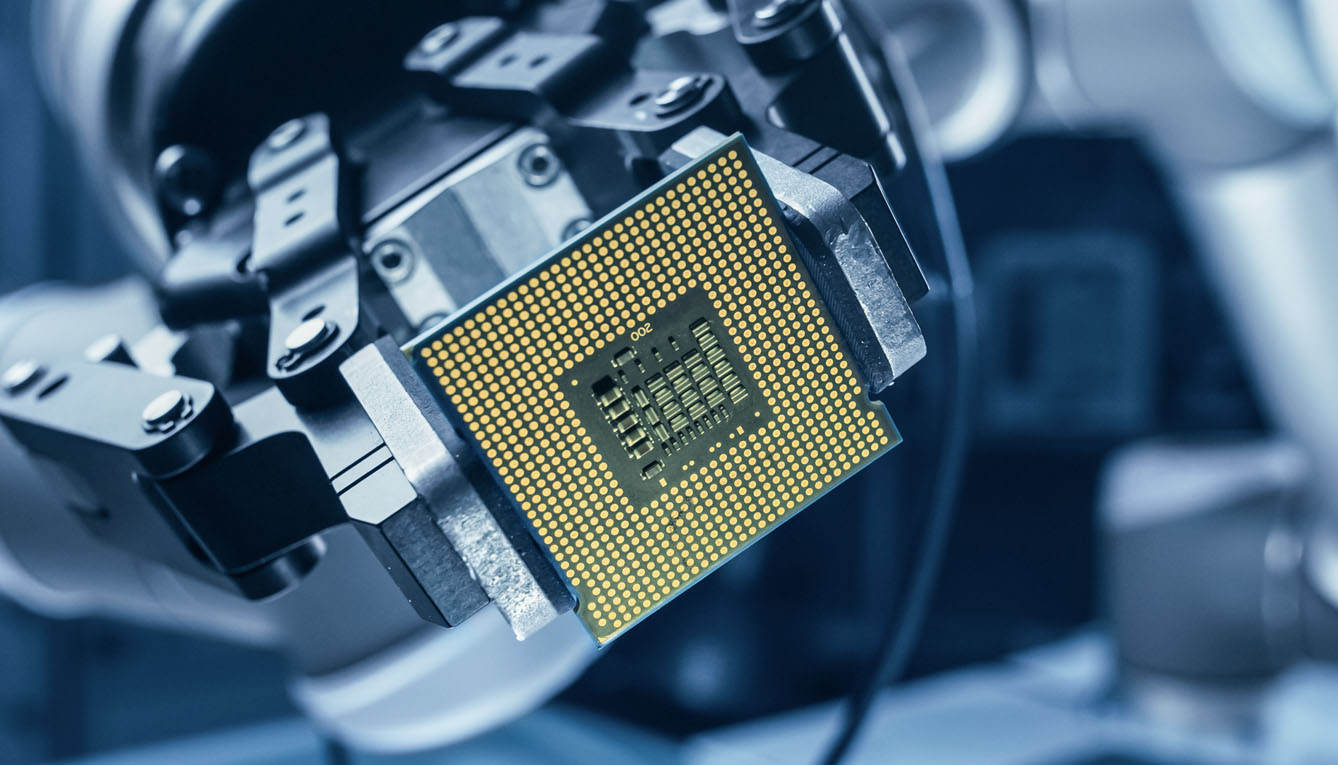
\includegraphics[width=\paperwidth, height=.5\paperheight]{picture1}};
	\end{tikzpicture}

	\vspace{13cm}
	\noindent \textcolor{myblue}{\fontsize{40pt}{40pt}\selectfont \textbf{Amplificador Diferencial}}\\\\
	{\fontsize{18pt}{18pt}\selectfont Julio, 2023} 
	
	\newpage
	\section*{Ampificador Diferencial}
	\subsection*{Funciones y características del amplificador operacional}
	El amplificador operacional está diseñado para sensar la diferencia entre las señales de voltaje aplicadas entre sus dos terminales de entradas (es decir, la cantidad $v_2-v_1$) multiplicada por un número A, causando un voltaje resultante $A(v_2-v_1)$ que aparece en la terminal de salida. Así $v_3=A(v_2-v_1)$. \\
	
	El amplificador operacional no consume ninguna corriente en la entrada, esto es, la señal de corriente en la terminal 1 y la señal de corriente en la terminal 2 son ambas cero. En otras palabras, la impedancia de entrada de un amplificador operacional ideal es infinita.
	Colocando junto todo lo anterior, llegamos al modelo de circuito equivalente mostrado en la figura \ref{fig:figura1}. Note que la salida está en fase con (tiene el mismo signo que)  $v_2$ y está en desfase con (tiene el signo opuesto de) $v_1$. Por esta razón, la terminal de entrada 1 es llamada terminal de entrada inversora y se distingue por el signo “-”, mientras que la terminal de entrada 2 es llamada terminal de entrada no inversora y se distingue por el signo “+”.
	
	\begin{figure}[H]
		\centering	
		\begin{tikzpicture}[]
			%\draw[step=1, gray,very thin] (-6.4,-6.4) grid (8.4,8.4);
			\draw[line width=0.5mm, fill=cyan!25] (0,0) -- (0,6) -- (26.56:6.71) -- (0,0);
			\draw (2.5,3) to[cV, invert, l_=$A(v_2 - v_1)$] (2.5,1);
			\draw (2.5,1) node[ground] {};
			%\draw (8,3) node[above]{$v_o$} to[short, -o] (3,3);
			\draw (2.5,3) to[short, -o] (6.5,3) node[right]{$v_o$};
			%\draw (4,4) node[above left] {$\bm{V_A}$};
			%\draw[->]  (6,5) -- (7.5,3.1);
			\draw [cyan,line width=0.5mm,-{Computer Modern Rightarrow[flex'=0.75]}]
			(7,4) .. controls (6.5,4) and (7,3.5) .. (6.5,3.2);
			\draw (7,4) node[cyan,above right] {output};
			\draw (-2,5) node[above right]{$1$} to [short, f_={$i_1 = 0$}, o-o] (0.5,5) node[right]{$-$};
			\draw (-2,1) node[above right]{$2$} to [short, f_={$i_2 = 0$}, o-o] (0.5,1) node[right]{$+$};
			\draw [cyan,line width=0.5mm,-{Computer Modern Rightarrow[flex'=0.75]}]
			(-1.5,6) .. controls (-1.6,5.5) and (-1.3,5.3) .. (-1.6,5.1);
			\draw (-1.5,6) node[cyan,above] {Inverting input};
			\draw [cyan,line width=0.5mm,-{Computer Modern Rightarrow[flex'=0.75]}]
			(-1,0) .. controls (-2,0.3) and (-2,0.6) .. (-2,0.9);
			\draw (-1,-0.2) node[cyan,below] {Noninverting input};
			\draw (-3,5) to[short, -o] (-2,5);
			\draw (-3,5) to[V, invert, l_=$v_1$] (-3,3);
			\draw (-3,3) node[ground] {};
			\draw (-3,1) to[short,-o] (-2,1);
			\draw (-3,1) to[V, invert, l_=$v_2$] (-3,-1);
			\draw (-3,-1) node[ground] {};
		\end{tikzpicture}
		\caption{Circuito equivalente del amplificador operacional ideal.}	
		\label{fig:figura1}
	\end{figure}
	
	De la descripción anteriormente vista, el amplificador operacional responde solo a la diferencia de la señal $v_2-v_1$ e ignora cualquier señal común a ambas entradas. Esto es, si $v_1=v_2=1$ V, entonces la salida será (idealmente) cero. A esta propiedad la llamamos \textbf{rechazo en modo común} y concluimos que el amplificador operacional ideal tiene una ganancia en modo común de cero. Así, la ganancia $A$ es llamada \textbf{ganancia diferencial}, por obvias razones. \\
	
	Una característica importante de los amplificadores operacionales es que estos están acoplados directamente o también llamados amplificadores de dc. Este hecho nos permite usarlos en muchas aplicaciones importantes, desafortunadamente, esta propiedad puede causarnos también algunos problemas serios.
	
	\subsection*{Señal diferencial y en modo común}
	La señal de entrada diferencial $v_{Id}$ es simplemente la diferencia entre las señales $v_1$ y $v_2$, esto es:
	
	\begin{align}
		v_{Id} = v_2 - v_1
	\end{align}
	
	La señal de entrada en modo común es el promedio de las dos señales de entrada $v_1$ y $v_2$:
	\begin{align}
		v_{Icm} = \frac{1}{2}(v_2 - v_1)
	\end{align}
	
	Las ecuaciones (1) y (2) pueden ser usadas para expresar las señales de entrada $v_1$ y $v_2$ en términos de la componente diferencial y de modo común. Despejando $v_2$ de la ecuación (2) obtenemos:
	
	\begin{align}
		v_2 = 2v_{Icm} - v_1
	\end{align}
	
	Sustituimos la ecuación (3) en la ecuación (1):
	\begin{align}
		v_{Id} &= 2v_{Icm} - v_1 - v_1\\
		v_{Id} &= 2v_{Icm} - 2v_1
	\end{align}
	
	Despejamos $v_1$ de la ecuación (5)
	\begin{tcolorbox}[colback=red!5!white,colframe=red!75!black,arc=0mm,boxrule=0mm,width=(\linewidth+0.5cm)]
		\begin{equation}
			v_1 = v_{Icm} - \frac{v_{Id}}{2}
		\end{equation}
	\end{tcolorbox}

	De igual manera
	\begin{tcolorbox}[colback=red!5!white,colframe=red!75!black,arc=0mm,boxrule=0mm,width=(\linewidth+0.5cm)]
		\begin{equation}
			v_2 = v_{Icm} + \frac{v_{Id}}{2}
		\end{equation}
	\end{tcolorbox}
	
	\begin{figure}[H]
		\centering	
		\begin{tikzpicture}[]
			%\draw[step=1, gray,very thin] (-6.4,-6.4) grid (8.4,8.4);
			\draw (0,0) to[V, l=$v_1$] (0,3);
			\draw (0,0) node[ground] {};
			\draw (0,3) to[blue!40, short, -o] node[above right]{1} (2,3); 
			\draw (0,-1) to[V, invert, l_=$v_1$] (0,-4);
			\draw (0,-4) node[ground] {};
			\draw (0,-1) to[blue!40, short, -o] node[above right]{2} (2,-1);
			\draw (3,0) node {$\equiv$} (3,0);
			\draw (4,1) to[V, invert, l=$v_{Icm}$]  (4,-2);
			\draw (4,1) to[short, -*] (7,1);
			\draw (7,1) to[V, invert, l_=$v_{Id}/2$] (7,4);
			\draw (7,4) to[blue!40, short, -o] (9,4) node[blue!40,above]{1};
			\draw (7,1) to[V, l=$v_{Id}/2$] (7,-2);
			\draw (7,-2) to[short, -o] (9,-2) node[blue!40, above]{2};
			\draw (4,-2) node[ground] {};
		\end{tikzpicture}
		\caption{Representación de las fuentes de señales $v_1$ y $v_2$ en términos de sus componentes diferencial y de modo común.}	
		\label{fig:figura2}
	\end{figure}
	
	\subsection*{Amplificadores diferenciales}
	Un amplificador de diferencias es uno que responde a la diferencia entre las dos señales aplicadas en sus entradas y rechaza las señales en que son comunes a ambas entradas. Así, idealmente el amplificador de diferencias amplificará sólo la señal de entrada diferencial $v_{Id}$ y rechazará completamente la señal de entrada en modo común $v_{Icm}$, los circuitos prácticos tendrán un voltaje de salida dado por:
	
	\begin{tcolorbox}[colback=red!5!white,colframe=red!75!black,arc=0mm,boxrule=0mm,width=(\linewidth+0.5cm)]
		\begin{equation}
			v_O = A_d v_{Id} + A_{cm} v_{Icm}
		\end{equation}
	\end{tcolorbox}
	
	Donde $A_d$ denota la ganancia diferencial y $A_{cm}$ denota la ganancia en modo común (idealmente cero). La eficacia de un amplificador diferencial se mide por el grado de su rechazo de las señales en modo común en preferencia a las señales diferenciales. Esto es usualmente cuantificado por una medición conocida como \textbf{razón de rechazo en modo común (CMRR)}, definido como
	
	\begin{tcolorbox}[colback=red!5!white,colframe=red!75!black,arc=0mm,boxrule=0mm,width=(\linewidth+0.5cm)]
		\begin{equation}
			CMRR = 20\log{\frac{|A_d|}{|A_{cm}|}}
		\end{equation}
	\end{tcolorbox}
	
	\subsubsection*{Ecuaciones de diseño}
	Nuestro primer esfuerzo en diseñar un amplificador operacional se ve motivado por la observación de que la ganancia de un amplificador en configuración no inversora es positiva, $(1+ R_2 / R_1 )$, mientras que la ganancia en la configuración inversora en negativa, $(-R_2 / R_1 )$. Con el fin de rechazar las señales en modo común debemos hacer que las dos magnitudes de las ganancias sean iguales, esto puede lograrse fácilmente atenuando la señal de entrada positiva con el fin  de reducir la ganancia de $(1+ R_2 / R_1 )$ a $(-R_2 / R_1 )$. El circuito resultante se muestra en la figura 3, donde la atenuación en el camino positivo se logra mediante un divisor de voltaje $(R_3,R_4 )$.
	
	\begin{figure}[H]
		\centering	
		\begin{tikzpicture}[]
			%\draw[step=.5, gray,very thin] (-6.4,-6.4) grid (8.4,8.4);
			\draw (0,0) node[op amp, anchor=+](OA){};
			\draw (OA.-) to[short] ++(-1,0) coordinate(node1) to[R, l_=$R_1$, -o] ++(-3,0) node[left]{$v_{i1}$};
			\draw (node1) to[short, *-] ++(0,2) coordinate (node2);
			\draw (node2) to[R, l=$R_2$] (node2 -| OA.out) -- (OA.out);
			\draw (OA.out) to[short, -*] (OA.out);
			\draw (OA.out) to[short, -o] ++(1,0) node[right]{$v_o$};
			\draw (OA.+) to[short, -*] ++(-1,0) coordinate(node4) to[R, l=$R_4$] ++(0,-3) node[ground]{};
			\draw (node4) to[R, l=$R_3$, -o] ++(-3,0) node[left]{$v_{i2}$};
			%	  (OA.-) to [R] (-2.5, 1);
			%\draw (0,0) to[short, -*] (0,0);
			%\draw (0,1) to[short, -*] ++(0,1);
		\end{tikzpicture}
		\caption{Amplificador Diferencial.}	
		\label{fig:figura3}
	\end{figure}
	
	\noindent Específicamente, deseamos determinar el voltaje de salida $v_o$ en términos de $v_{I1}$ y $v_{I2}$. Observamos que el circuito es linear por lo que podemos usar el método de superposición.\\
	
	\noindent Para aplicar el método de superposición, primero reducimos $v_{I2}$ a cero, esto es, aterrizamos el terminal donde se conecta $v_{I2}$ y entonces encontramos el voltaje de salida correspondiente el cual estará en términos de  $v_{I1}$. Denotamos este voltaje de salida como $v_{O1}$. Su valor puede encontrarse del circuito de la figura 4 en el cual reconocemos como una configuración inversora. La existencia de $R_3$ y $R_4$ no afecta la expresión de la ganancia dado que la corriente no fluye a través de estas. Así
	
	\begin{tcolorbox}[colback=red!5!white,colframe=red!75!black,arc=0mm,boxrule=0mm,width=(\linewidth+0.5cm)]
		\begin{equation}
			v_{O1} = -\frac{R_2}{R_1}v_{i1}
		\end{equation}
	\end{tcolorbox}
	
	\begin{figure}[H]
		\centering	
		\begin{tikzpicture}[scale=0.8]
			%\draw[step=.5, gray,very thin] (-6.4,-6.4) grid (8.4,8.4);
			\draw (0,0) coordinate(A) node[op amp, anchor=+](OA){};
			\draw (OA.-) to[short] ++(-1,0) coordinate(node1) to[R, l_=$R_1$, -o] ++(-3,0) node[left]{$v_{i1}$};
			\draw (node1) to[short, *-] ++(0,2) coordinate (node2);
			\draw (node2) to[R, l=$R_2$] (node2 -| OA.out) -- (OA.out);
			\draw (OA.out) to[short, -*] (OA.out);
			\draw (OA.out) to[short, -o] ++(1,0) node[right]{$v_{o1}$};
			\draw (OA.+) to[short, -*] ++(-1,0) coordinate(node4) to[R, l=$R_4$] ++(0,-3) node[ground]{};
			\draw (node4) to[short] ++(-2,0) to[R, l=$R_3$] ++(0,-3) node[ground]{};
			
			
			\draw (A) ++(10,0) coordinate(B) node[op amp, anchor=+](OA1){};
				\draw (OA1.-) to[short] ++(-1,0) coordinate(nodeA) to[R, l_=$R_1$,] ++(-3,0) node[ground]{};
				\draw (nodeA) to[short, *-] ++(0,2) coordinate (nodeB);
				\draw (nodeB) to[R, l=$R_2$] (nodeB -| OA1.out) -- (OA1.out);
				\draw (OA1.out) to[short, -*] (OA1.out);
				\draw (OA1.out) to[short, -o] ++(1,0) node[right]{$v_{o2}$};
				\draw (OA1.+) to[short, -*] ++(-1,0) coordinate(nodeC) to[R, l=$R_4$] ++(0,-3) node[ground]{};
				\draw (nodeC) to[R, l=$R_3$, -o] ++(-3,0) node[left]{$v_{i2}$};
		\end{tikzpicture}
		\caption{Aplicación del método de superposición para analizar el circuito de la figura 3}	
		\label{fig:figura4}
	\end{figure}
	
	\noindent Ahora reducimos $v_{I1}$ a cero y evaluamos el correspondiente voltaje de salida $v_{O2}$. El circuito toma ahora la forma mostrada en la figura 5 la cual reconocemos como una configuración no inversora con un divisor de voltaje adicional constituido por $R_3$ y $R_4$ las cuales están conectadas a la entrada $v_{I2}$. El voltaje de salida $v_{O2}$ está entonces dado por:
	
	\begin{tcolorbox}[colback=red!5!white,colframe=red!75!black,arc=0mm,boxrule=0mm,width=(\linewidth+0.5cm)]
		\begin{equation}
			v_{O2} = v_{I2}\frac{R_4}{R_3 + R_4}\left( 1 + \frac{R_2}{R_1} \right)
		\end{equation}
	\end{tcolorbox}
	
	El principio de superposición nos dice que el voltaje de salida $v_O$ es igual a la suma de $v_{O1}$ y $v_{O2}$. Así tenemos:
	\begin{tcolorbox}[colback=red!5!white,colframe=red!75!black,arc=0mm,boxrule=0mm,width=(\linewidth+0.5cm)]
		\begin{equation}
			v_{O} = v_{I2}\frac{R_4}{R_3 + R_4}\left( 1 + \frac{R_2}{R_1} \right) - \frac{R_2}{R_1}v_{I1}
		\end{equation}
	\end{tcolorbox}
	
	\subsection*{Análisis del amplificador operacional con entrada en modo común}
	\noindent Ahora consideraremos el circuito con una señal de entrada en modo común aplicada en la entrada, como se muestra en la figura 5.
	
	\begin{figure}[H]
		\centering	
		\begin{tikzpicture}[]
			%\draw[step=.5, gray,very thin] (-6.4,-6.4) grid (8.4,8.4);
			\draw (0,0) node[op amp, anchor=+](OA){};
			\draw (OA.-) to[short] ++(-1,0) coordinate(nodeC) to[R, l_=$R_1$, f_<=$i_1$] ++(-3,0) coordinate(nodeA);
			\draw (OA.+) to[short] ++(-1,0) coordinate(nodeD) to[R, l_=$R_3$] ++(-3,0) coordinate(nodeB);
			\draw (nodeA) to[short] (nodeB);
			\draw (nodeD) to[R, l=$R_4$, *-] ++(0,-3) node[ground]{};
			\draw (nodeC) to[short, *-] ++(0,2) coordinate(nodeE);
			\draw (nodeE) to[R, l=$R_2$, f>^=$i_2$] (nodeE -| OA.out) -- (OA.out);
			\draw (OA.out) to[short, *-o] ++(1,0) node[right]{$v_o$};
			\coordinate (M) at ($(nodeA)!0.5!(nodeB)$);
			\draw (M) to[short, *-] ++(-1,0)
				to[V, invert, l_=$v_{Icm}$] ++(0,-3) node[ground]{};
			\draw (-3,-2) node[cyan]{$\left( \frac{R_4}{R_3 + R_4} \right)v_{Icm}$} coordinate(equ);
			\coordinate (nodeCp1) at ($(nodeC)!0.1!(nodeD)$);
			\coordinate (nodeCp2) at ($(nodeC)!0.9!(nodeD)$);
			\draw [cyan, ->] ($(equ)+(0.1,0.4)$) -- (nodeCp1);
			\draw [cyan, ->] ($(equ)+(0.2,0.4)$) -- ($(nodeCp2)+(-0.1,-0.2)$);
		\end{tikzpicture}
		\caption{Amplificador Diferencial.}	
		\label{fig:figura5}
	\end{figure}
	
	\noindent Aplicando la LCK en el nodo $v_-$ obtenemos:
	\begin{align*}
		i_1 = 1_2
	\end{align*}
	
	\noindent O bien
	\begin{align*}
		\frac{v_{Icm}- v_-}{R_1} = \frac{v_- - v_o}{R_2}
	\end{align*}
	
	\begin{align}
		\left( \frac{1}{R_1} + \frac{1}{R_2} \right)v_- = \frac{v_{Icm}}{R_1} + \frac{v_o}{R_2}
	\end{align}
	
	\noindent Ahora aplicamos la LCK en el nodo $v_+$
	\begin{align*}
		i_3 = i_4
	\end{align*}
	
	\noindent O bien
	\begin{align*}
		\frac{v_{Icm}- v+}{R_3} = \frac{v_+}{R_4}\\
		\frac{v_{Icm}}{R_3} - \frac{v_+}{R_3} = \frac{v_+}{R_4}\\
		\left( \frac{1}{R_3} + \frac{1}{R_4} \right)v_+ = \frac{v_{Icm}}{R_3}\\
		\left( \frac{R_3 + R_4}{R_3R_4} \right)v_+ = \frac{v_{Icm}}{R_3}
	\end{align*}
	
	\noindent Despejamos $v_+$ de la ecuación anterior
	\begin{align}
		v_+ = \frac{R_4}{R_3 + R_4}v_{Icm}
	\end{align}
	
	\noindent Sin embargo, tenemos que $v_- = v_+$, así, sustituimos la ecuación (14) en (13)
	\begin{align}
		\left( \frac{1}{R_1} + \frac{1}{R_2} \right) \left( \frac{R_4}{R_3 + R_4} \right)v_{Icm} = \frac{v_{Icm}}{R_1} + \frac{v_o}{R_2}\nonumber
	\end{align}
	
	\begin{align}
		\left[ \left( \frac{R_1 + R_2}{R_1R_2} \right)\left( \frac{R_4}{R_3 + R_4} \right) - \frac{1}{R_1} \right]v_{Icm} = \frac{v_o}{R_2}\nonumber
	\end{align}  
	
	\begin{align}
		\frac{R_1R_4 + R_2R_4 - R_2R_3 - R_2R_4}{R_1R_2(R_3 + R_4)}v_{Icm} = \frac{v_o}{R_2}\nonumber
	\end{align}

	\noindent Al despejar $v_o$ de la ecuación anterior obtenemos	
	\begin{align}
		v_o = \frac{R_1R_4 - R_2R_3}{R_1(R_3 + R_4)}v_{Icm} = \left[ \frac{R_4}{R_3 + R_4} - \frac{R_2R_3}{R_1(R_3 + R_4)} \right]v_{Icm}
	\end{align}
	
	\noindent La ganancia en modo común es:
	\begin{tcolorbox}[colback=red!5!white,colframe=red!75!black,arc=0mm,boxrule=0mm,width=(\linewidth+0.5cm)]
		\begin{equation}
			A_{cm} = \frac{v_o}{v_{Icm}} = \frac{R_4}{R_3 + R_4}\left( 1 - \frac{R_2}{R_1} \frac{R_3}{R_4} \right)
		\end{equation}
	\end{tcolorbox}
	
	\noindent Para que la ganancia en modo común sea igual a cero, debemos hacer que el cociente $(R_2R_3)/(R_1R_4)$ sea igual a 1, lo cual podemos lograr haciendo
	\begin{align}
		R_3 = R_1 \quad \quad R_4 = R_2
	\end{align}
	
	\noindent Con estos valores, la ganancia en modo común sería entonces
	\begin{align}
		A_{cm} = 0
	\end{align}
	
	Note, sin embargo, que cualquier discordancia entre el cociente de los resistores puede hacer que $A_{cm}$ sea diferente de cero y por lo tanto un CMRR finito. Si sustituimos (17) en (12) obtenemos
	\begin{tcolorbox}[colback=red!5!white,colframe=red!75!black,arc=0mm,boxrule=0mm,width=(\linewidth+0.5cm)]
		\begin{equation}
			v_o = \frac{R_2}{R_1 + R_2}\left( \frac{R_1 + R_2}{R_1} \right)v_{I2} - \frac{R_2}{R_1}v_{I1} = \frac{R_2}{R_1} \left( v_{I2} - v_{I1} \right)
		\end{equation}
	\end{tcolorbox}	
\end{document}